\cleardoublepage
\addcontentsline{toc}{chapter}{ANEXOS}
\section*{ANEXOS}

\appendix
\renewcommand{\thesection}{Anexo \Alph{section}} 
\addtocontents{toc}{\protect\fixAnexoToc}

\section{Repositorio GitHub}
\label{anexo:github}

\begin{figure}[htbp]
    \centering
    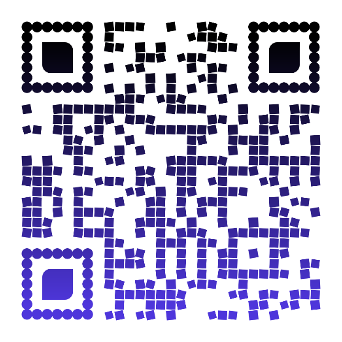
\includegraphics[width=0.8\linewidth]{imagenes/Repositorio.png}
    \caption{Repositorio de Github}
    \label{fig:repo_qr}
\end{figure}

\section{Cuestionario a usuarios}
\label{anexo:Cuestionarios}
Se realizaron cuestionarios a los usuarios del sistema, los cuestionarios fueron adaptados a el area correspondiente de cada usuario.
\subsection{Cuestionario a Administradores}
 \begin{enumerate}
     \item ¿Qué tan eficiente considera la generación de reportes administrativos en comparación con el manejo anterior en Excel?
    \item ¿El sistema le permite identificar con claridad las discrepancias en el inventario de hologramas en tiempo real?
    \item ¿Cómo califica la utilidad de las alertas de la bóveda para la planeación de la logística de hologramas?
    \item ¿Considera que el módulo administrativo facilita el seguimiento contable de los movimientos diarios del verificentro?
    \item ¿Qué funcionalidad adicional de supervisión agregaría para mejorar el control de las operaciones?
\end{enumerate}

\subsection{Cuestionario a Usuarios de Captura}
\begin{enumerate}
    \item ¿Qué tan intuitiva resulta la interfaz de captura comparada con el uso de hojas de cálculo de Excel?
    \item ¿El sistema le ayuda a prevenir errores de dedo mediante validaciones automáticas durante el ingreso de datos?
    \item ¿Considera que el diseño de las vistas de captura es ergonómico para jornadas de trabajo prolongadas?
    \item ¿Qué proceso manual que aún realiza cree que debería integrarse totalmente a esta vista?
\end{enumerate}

\subsection{Cuestionario a usuarios modulo Caja}
\begin{enumerate}
    \item ¿Cómo ha cambiado el tiempo de captura de información interna en el sistema comparado con el proceso anterior?
    \item ¿El flujo de recepción de documentos en "puerta" se integra de manera fluida con el registro en el módulo de caja?
    \item ¿Qué tan claros son los reportes de corte de caja que genera el sistema al final del turno?
    \item ¿Ha experimentado errores en la validación de datos durante la captura que el sistema no haya detectado?
    \item ¿La interfaz le permite gestionar los pagos de forma rápida para evitar cuellos de botella en la atención?
\end{enumerate}

\subsection{Cuestionario usuarios modulo Entrega de resultados}
\begin{enumerate}
    \item ¿Cómo califica la efectividad de las alertas al momento de preparar la entrega del resultado y el holograma?
    \item ¿El proceso de generación del reporte final de resultados es más ágil que cuando se realizaba manualmente?
    \item ¿Ha notado una disminución en los errores de entrega de hologramas desde la implementación de SIVEH?
    \item ¿La vista de entrega le proporciona toda la información necesaria sobre el estado del vehículo sin tener que navegar a otros módulos?
    \item ¿El sistema facilita la comunicación con el área de caja en caso de que existan pendientes antes de la entrega?
\end{enumerate}

\subsection{Cuestionario UX/UI}
\begin{enumerate}
    \item ¿La paleta de colores del sistema facilita la lectura y el enfoque en las tareas importantes?
    \item ¿Considera que la disposición de los menús y botones es lógica y fácil de aprender para nuevos usuarios?
    \item En una escala del 1 al 10, ¿qué tan amigable le resulta el sistema en comparación con las herramientas anteriores (Excel/Manual)?
    \item ¿El tiempo de respuesta del sistema al generar reportes o procesar capturas es el adecuado para el flujo del verificentro?
    \item ¿Cuál es su nivel de confianza al usar el sistema para realizar sus actividades diarias sin temor a perder información?
\end{enumerate}

\section{Manuales}
A continuacion se presentan los codigos QR para acceder a los manuales necesarios para uso del sistema.
\subsection{Manual Tecnico}
\begin{figure}[htbp]
    \centering
    
\includegraphics[width=0.5\linewidth]{imagenes/QR Manual Tecnico.png}
    \caption{Manual Tecnico}
    \label{fig:manualtec_qr}
\end{figure}

\subsection{Manual de Usuario}
\begin{figure}[htbp]
    \centering
    
\includegraphics[width=0.5\linewidth]{imagenes/QR Manual Usuario.png}
    \caption{Manual de Usuario}
    \label{fig:manualuser_qr}
\end{figure}

\section{Tablas de Base de datos}
\label{anexo:Tablas BD}

\subsection{Tabla Catálogos Taller}
\begin{figure}[htbp]
    \centering
    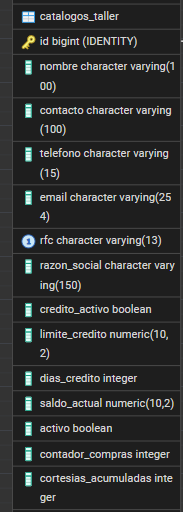
\includegraphics[width=0.5\linewidth]{imagenes/cstalogo talleres.png}
    \caption{Catalogo Talleres}
    \label{fig:tabla Talleres}
\end{figure}
Almacena la información detallada de los talleres externos vinculados al verificentro. Contiene datos de identificación legal, información de contacto y campos específicos para la gestión financiera, como límites de crédito, saldos actuales y el seguimiento de cortesías acumuladas por volumen de compra.

\subsection{Tabla Catálogos Técnico}
\begin{figure}[htbp]
    \centering
    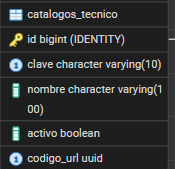
\includegraphics[width=0.5\linewidth]{imagenes/cstalogo tecnico.png}
    \caption{Catalogo Tecnicos}
    \label{fig:tabla Tecnicos}
\end{figure}
Entidad destinada al registro del personal técnico encargado de realizar las pruebas de verificación. Incluye una clave de identificación única por técnico y un campo \texttt{codigo\_url} de tipo UUID, utilizado para la generación de enlaces seguros o identificación digital dentro del sistema SIVEH.





\section{Tarjetas Kanban y Migraciones}
\label{anexo:kanban-migraciones}

\begin{center}
\begin{tabular}{|c|p{5.5cm}|l|}
\hline
\textbf{Tarjeta} & \textbf{Descripción} & \textbf{Estado Final} \\
\hline
K-01 & Schema inicial: subsistemas, usuarios, matrícula, evaluaciones, titulación & Desplegado \\
K-02 & Carga de catálogo de 7 subsistemas educativos & Desplegado \\
K-03 & Campos de auditoría en trabajos de carga & Desplegado \\
K-04 & Corrección de longitud en columna de estado & Desplegado \\
K-05 & Rol directivo y bitácora de auditoría & Desplegado \\
K-06 & Configuración de mapeo de columnas en Excel & Desplegado \\
K-07 & Renombrado y redefinición de roles del sistema & Desplegado \\
K-08 & Módulo de caracterización (discapacidad y etnia) & Desplegado \\
K-09 & Módulo de becas estudiantiles & Desplegado \\
K-10 & Catálogo de ciclos generacionales válidos & Desplegado \\
K-11 & Corrección semántica de campo docente & Desplegado \\
K-12 & Ajuste de campos nulos en titulación & Desplegado \\
K-13 & Desglose por sexo en becas y caracterización & Desplegado \\
\hline
\end{tabular}
\end{center}